\begin{frame}
    \frametitle{Barriers in a Waste Repository}
    The main constraint for loading of a waste repository is the \textbf{thermal constraint} set by the material properties of the repository. 
    \\
    \begin{figure}[htbp!]
      \begin{center}
        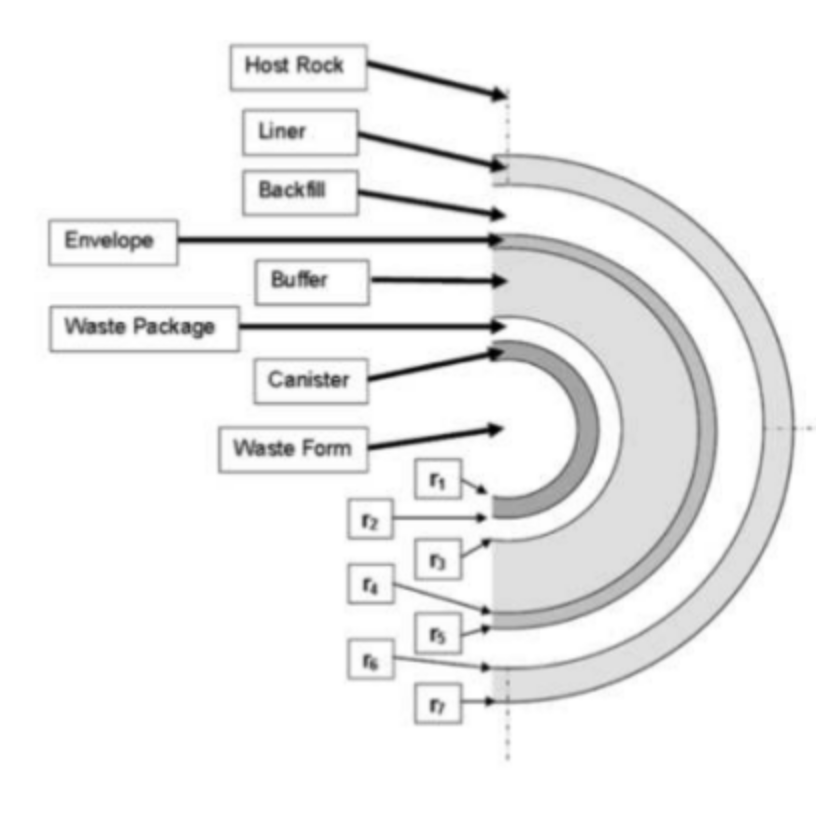
\includegraphics[height=5cm]{../figures/barriers}
      \end{center}
            \caption{Layers of Waste Repository Barrier System }
    \end{figure}
  \end{frame}

\begin{frame}
    \frametitle{Heat Flux through Barriers in a Waste Repository}
    
    Waste package thermal evolution depends on the \textbf{decay heat contribution from each isotope} in the spent fuel. 
    \\
    \begin{columns}
      \column[t]{5cm}
    \begin{figure}[htbp!]
      \begin{center}
        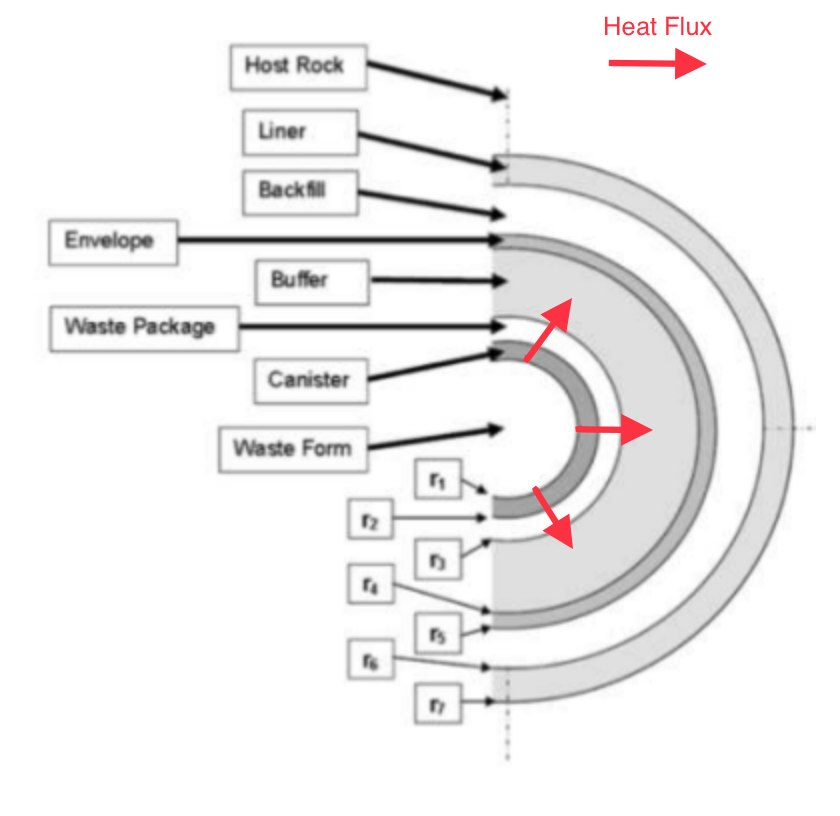
\includegraphics[height=4.3cm]{../figures/barriers_annotated}
      \end{center}
            \caption{Layers of Waste Repository Barrier System }
    \end{figure}
    \column[t]{5cm}
    Significant isotopes for \textbf{long term} decay heat contribution \cite{wigeland_separations_2006}
    \begin{itemize}
      \item $^{240}$Pu
      \item $^{241}$Am
      \item $^{239}$Pu
    \end{itemize}
    Significant isotopes for \textbf{short term} decay heat contribution \cite{wigeland_separations_2006}
    \begin{itemize}
      \item $^{238}$Pu
      \item $^{244}$Cm
      \item $^{90}$Sr
      \item $^{137}$Cs
    \end{itemize}
    \end{columns}
  \end{frame}

  \begin{frame}
    \frametitle{Motivation for conducting the Validation}

    \textbf{Reason for Validation:} 
    \\
    
    Check if the cyclus simulation gives total spent fuel masses and isotopic compositions that closely replicates reality. 

    \begin{figure}[htbp!]
      \begin{center}
        
\includegraphics[height=2cm]{../figures/accuracy_flow}
      \end{center}
            \caption{Accurate simulations for loading of a waste repository relies on accurate heat flux and isotopic composition information}
    \end{figure}

  \end{frame}
  